\documentclass[a4paper,oneside,12pt]{book}

%----------------------------------------------------------------------------------------
%	README!
%   Welcome. It's worth having a read through this file
%   to set up the broad parameters, such as the name of
%   the degree, the school/department, the type of work
%   (dissertation/Final Year Project/report, etc. as well
%   as your own details.
%----------------------------------------------------------------------------------------

%----------------------------------------------------------------------------------------
%	COVER PAGE
%   The cover page is laid out in title/title.tex. You can choose a colour
%   or black and white logo
%----------------------------------------------------------------------------------------

%----------------------------------------------------------------------------------------
%	THESIS INFORMATION
%   Put title, author name, degree, type of work, school, department in here
%   It will be used for the title page and for the embedded PDF information
%----------------------------------------------------------------------------------------

\newcommand{\thesistitle}{Entitlement Methods \textendash\ \\An Example of the Great Famine in Ireland, 1845 \textendash\ 1851} % Your thesis title, this is used in the title and abstract
\newcommand{\degree}{M.Sc. Applied Social Data Sciences} % Your degree name, this is used in the title page and abstract
\newcommand{\typeofthesis}{Dissertation} % dissertation, Final Year Project, report, etc.
\newcommand{\authorname}{Chenxi Li} % Your name, this is used in the title page and PDF stuff
%% Do not put your Student ID in the document, as TCD will not publish
%% documents that contain both your name and your Student ID.
\newcommand{\authorid}{23330541}
\newcommand{\keywords}{this, that, more} % Keywords for your thesis
\newcommand{\school}{\href{https://www.tcd.ie/Political_Science/}{School of Political}} % Your school's name and URL, this is used in the title page

%% Comment out the next line if you don't want a department to appear
%\newcommand{\department}{\href{http://researchgroup.university.com}{Prof. Peter Dunne}} % Your research group's name and URL, this is used in the title page

\AtBeginDocument{
\hypersetup{pdftitle=\thesistitle} % Set the PDF's title to your title
\hypersetup{pdfauthor=\authorname} % Set the PDF's author to your name
\hypersetup{pdfkeywords=\keywords} % Set the PDF's keywords to your keywords
\hypersetup{pdfsubject=\degree} % Set the PDF's keywords to your keywords
}

%% Language and font encodings
\usepackage[T1]{fontenc} 
\usepackage[utf8]{inputenc}
\usepackage[english]{babel}
\usepackage{ragged2e} %allows for text alignment preferences

%% Bibliographical stuff
\usepackage[round,sort,comma]{natbib}
\usepackage[hang, bottom]{footmisc} % no space in footnote

%% Document size
% include showframe as an option if you want to see the boxes
\usepackage[a4paper, top=2.56cm,bottom=2.56cm,left=2.56cm,right=2.56cm, head = 16pt]{geometry}
\setlength{\marginparwidth}{2cm}
%% Useful packages
\usepackage{amsmath}
\usepackage[autostyle=true]{csquotes} % Required to generate language-dependent quotes in the bibliography
\usepackage[pdftex]{graphicx}
\usepackage[colorinlistoftodos]{todonotes}
\usepackage[colorlinks=true, allcolors=black]{hyperref}
\usepackage{xcolor}
\usepackage{caption} % if no caption, no colon
%\usepackage{sfmath} %use sans-serif in the maths sections too
\usepackage[parfill]{parskip}    % Begin paragraphs with an empty line rather than an indent
\usepackage{setspace} % to permit one-and-a-half or double spacing
\usepackage{enumerate} % fancy enumerations like (i) (ii) or (a) (b) and suchlike
\usepackage{booktabs} % To thicken table lines
\usepackage{fancyhdr}

%\pagestyle{plain} % Embrace simplicity!

%% The Mechanical engineers require your name and ID on the top of every page.
%% Uncomment the following block if you want your name and ID at the top of
%% (almost) every page.

\pagestyle{fancy}
\fancyhf{} % sets both header and footer to nothing
\renewcommand{\headrulewidth}{0pt}
\cfoot{\thepage}
%\ifdefined\authorid
%\chead{\it \authorname\ (\authorid)}
%\else
%\chead{\it \authorname}
%\fi
%% End of block

%% It is not a requirement of the university that the font should be sans-serif, but
%% the Mechanical engineers require it. Comment out the following line to disable it
%%\renewcommand{\familydefault}{\sfdefault} %use the sans-serif font as default

%% If you're not using sans-serif, consider using Palatino instead of the LaTeX standard
\usepackage{mathpazo} % Use the Palatino font by default if you prefer it to Computer Modern

\renewcommand{\theequation}{\arabic{equation}} %% use continuous equation numbers

%% Format Chapter headings appropriately
\usepackage{titlesec}
\definecolor{tcdblue}{cmyk}{0.94, 0.38, 0, 0.27}
\newcommand{\hsp}{\hspace{5pt}}
\titleformat{\chapter}[hang]{\LARGE\bfseries}{\thechapter\hsp\textcolor{tcdblue}{|}\hsp}{0pt}{\LARGE\bfseries}
\titlespacing{\chapter}{0pt}{10pt}{0pt}

\title{\thesistitle}
\author{\authorname}

\frontmatter
\begin{document}
\begin{titlepage}

    \center % Center everything on the page
    
    %% All the text parameters should be taken from the start of the main.tex file.
    %% You should only alter stuff here if you want to change the layout
    
    %----------------------------------------------------------------------------------------
    %	LOGO SECTION
    %----------------------------------------------------------------------------------------
    %% Choose one of the following -- a colour or black-and-white logo
    
    
\includegraphics{title/Trinity_RGB_transparent_main.png}\\[1cm] 
    %
\includegraphics[width=12cm]{title/black-stacked-trinity.jpg}\\[1cm] 
    \ifdefined\school
    \Large \textsc{\school} \\[1.5cm] % Minor heading such as course title
    \ifdefined\department
    \large \department\\[1.5cm] % Minor heading such as course title
    \fi
    
    %----------------------------------------------------------------------------------------
    %	TITLE SECTION
    %----------------------------------------------------------------------------------------
    \makeatletter
    \textsc{{\huge \bfseries \thesistitle}}\\[1.5cm] % Title of your document
     
    
    %----------------------------------------------------------------------------------------
    %	AUTHOR SECTION
    %----------------------------------------------------------------------------------------
   
    \authorname
    \par
    \authorid
    
    %----------------------------------------------------------------------------------------
    %	DATE SECTION
    %----------------------------------------------------------------------------------------
    
    \textsc{{\large \today}}\\[2cm] % Date, change the \today to a set date if you want to be precise
    
    {School of Social Sciences and Philosophy, TCD}
    %----------------------------------------------------------------------------------------
    %	TYPE OF THESIS SECTION
    %----------------------------------------------------------------------------------------
    \vfill
    
    \textsc{\normalsize Submitted in partial fulfilment of the requirements for the degree of \\
    \degree}
    
    \vfill % Fill the rest of the page with whitespace
    
\end{titlepage}
\pagenumbering{roman}
\doublespacing

\newpage

\section*{Declaration}
I hereby declare that this \typeofthesis\ is entirely my own work and that it has not been submitted as an exercise for a degree at this or any other university.

I have read and I understand the plagiarism provisions in the General Regulations of the University Calendar for the current year, found at \url{http://www.tcd.ie/calendar}.

I have also completed the Online Tutorial on avoiding plagiarism 'Ready Steady Write', located at \url{http://tcd-ie.libguides.com/plagiarism/ready-steady-write}.

\vspace{.3cm}
\rule{10cm}{.3pt}

\begin{flushleft}
	\begin{minipage}{0.5\linewidth}
		\textbf{Signature:} 
		\raisebox{-0.3\height}{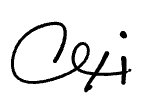
\includegraphics[width=0.6\linewidth]{signature.png}}
	\end{minipage}
\end{flushleft}
\textbf{Date: } \today
\vspace{.3cm}

\newpage

\section*{Acknowledgements}
I would like to thank my supervisor, \textbf{Prof. Martina Kirhberger}, for her guidance through each stage of this dissertation.

\chapter{Abstract}
A short summary of the problem investigated, the approach taken and the key findings. This should not be more that around 400 words.

The must be on a separate page.

\newpage
%\raggedright %\raggedright turns off justification and hypenation

\newpage \tableofcontents
\newpage \listoffigures
\newpage \listoftables

\newpage

\vspace{2cm}

\mainmatter
\chapter{Introduction}
\textit{October playing a symphony on a slack wire paling.\\
Maguire watches the drills flattened out\\
And the flints that lit a candle for him on a June altar,\\
Flameless. \\
\textemdash\ ``The Great Hunger'' by Patrick Kavanagh.} \citep{Kavanagh_Quinn_2006a}
\vspace{.2cm}

The Irish Great Famine (1845 \textendash\ 1852) reshaped the entire history of Ireland. Before the Great Famine, according to the 1841 census, the population of the Ireland had close to 8.5 million
\footnote{
	\href{https://www.cso.ie/en/statistics/historicalreports/census1841/}{1841 Census of Ireland, Last accessed: 13 May, 2024}
}
. In 1851, when the Irish Great Famine had not yet ended, census noted that about 1 million people had died for hunger, and a similar number had gone into overseas exile
\footnote{
	\href{https://www.cso.ie/en/statistics/historicalreports/census1851/}{1851 Census of Ireland, Last accessed: 2 May, 2024}
}. In 1926, as a result of the Irish independence 5 years earlier, the Central Statistical Office was capable to integrate historical documents since famine and showed the fact that the population was decline of roughly 22\%
\footnote{
	\href{https://www.cso.ie/en/media/csoie/census/census1926results/volume10/C_1926_V10_Chapter_II.pdf}{1926 Census of Ireland, Chapter II, Last acceseed: 9 May, 2024}
} in the 10 years from 1841 to 1851. Using parish baptism data, some scholars have estimated that in the year 1847 alone \textendash\ which is also known as black'47 in Ireland history \textendash\ there existed counties with a nearly 70\% reduction in baptisms in Munster province in the south of Ireland \citep{cousens1960regional}, especially from southwest Cork and including north and east Clare
\footnote{
	\href{https://www.rte.ie/history/the-great-irish-famine/2020/0629/1150367-the-great-irish-famine/}{RTE, How "a truly modern famine" devastated Ireland, Last accessed: 11 May, 2024}
}
, while it was not the worst hit by the famine compared to the province of Connacht in the west
\footnote{
	\href{https://www.wesleyjohnston.com/users/ireland/past/famine/summer_1847.html}{Wesley Johnston: The Famine: The Summer of Black'47, Last accessed: 13 May, 2024}
}
. Apart from these quantitative explorations, the Great Famine is equally pivotal in Irish cultural history and ethnography. From Joseph O'Connor's fiction ``Star of the sea'' to W. B. Yeats's ``The Countess Cathleen'', together they expressed that the Great Famine not only pointed to the corpses of the dead, but also to a black hole of identity, naming and meaning \citep{luchen41naming}. 

The effects of the Great Famine were far-reaching, and reflected in the long-term population development, land institution structure and attitude to the UK government directly. It was not until 120 years later, in the 1960s, that Ireland's population began to grow consistently due to large-scale emigration, late marriage and a high incidence of permanent celibacy no longer hold \citep{grada1979population}, but it was still nowhere near as large as it had been during the Great Famine
\footnote{
	\href{https://www.cso.ie/en/releasesandpublications/ep/p-cpsr/censusofpopulation2022-summaryresults/populationchanges/}
	{2022 Census of Ireland \textendash\ Summary Results, Last accessed: 8 May, 2024}
}.
This also makes Ireland one of the few countries in the world to suffer population decline over the past 170 years when the world's population has increased more than six fold
\footnote{
	\href{https://www.dfa.ie/irish-embassy/usa/about-us/ambassador/ambassadors-blog/black47irelandsgreatfamineanditsafter-effects/}
	{Blog by Ambassador Mulhall on Black'47: Ireland's Great Famine and its after-effects, Last accessed: 9 May, 2024}
}. Regarding the land, on the one hand, in the aftermath of the famine, there was a tendency in Ireland to shift from agriculture to livestock husbandry
\footnote{
	\href{https://www.cso.ie/en/statistics/othercsopublications/farmingsincethefamine1847-1996/}{CSO: Farming Since the Famine, 1847 - 1996, Last accessed: 12 May, 2024}
}, and on the other hand, when the late blight back in the 1870s, the Land War, which was directed at the landowners and the government, took place at the same time, with a deep consequences for the land structure of Ireland. Also, there raised hostility between Irish and UK government, which was described as ``a bankruptcy of the British-Irish Union of 1800'' \citep{gray2021great}.





People believe potato blight was responsible for the Irish Great Famine. 

lumper potato

Blight became a semi-permanent fixture until the end of the century, when effective treatments were found \citep{o1994economic}.

\bibliographystyle{agsm}
\bibliography{reference}

\appendix
\renewcommand{\thechapter}{A\arabic{chapter}}



\end{document}